\section{Überblick über die Verfahren}

Passende manuelle Verfahren gibt es für verschiedene Aufgabenstellungen und Teamgrößen: Besteht das Team nur aus wenigen Personen, reicht i.d.R. ein \textbf{Gutachter}.\\
Muss ein wichtiges Dokument geprüft werden (Anforderungsdokument als Vertragsgrundlage, zentraler, sicherheitskritischer Code), untersuchen mehrere Personen systematisch den Prüfgegenstand.\\

\noindent
Verschiedene Verfahren lassen sich nach der Anzahl der Teilnehmer und dem Umfang der Untersuchung einordnen (s. Abbildung~\ref{fig:manuelleverfahren} sowie Abschnitt~\ref{sec:andere-verfahren}).

\begin{figure}
    \centering
    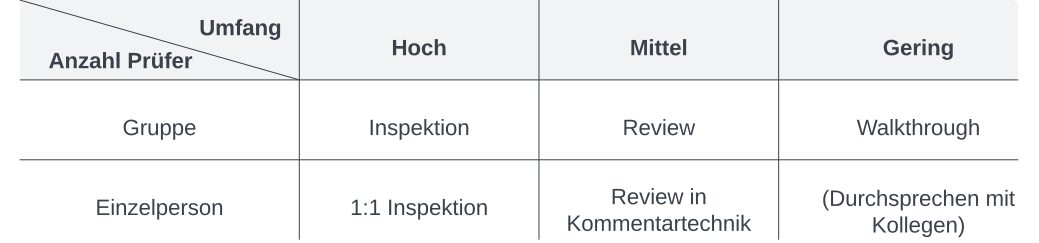
\includegraphics[scale=0.4]{part four/Manuelle Verfahren/img/manuelleverfahren}
    \caption{Verschiedene manuelle Verfahren, eingeordnet nach Anzahl der Teilnehmer und Umfang der Untersuchung. (Quelle: in Anlehnung an~\cite[Tab. 3.1, 17]{Wed09c})}
    \label{fig:manuelleverfahren}
\end{figure}

\noindent
\textbf{Inspektionen}, \textbf{Reviews} und \textbf{Walkthroughs} werden in Gruppen durchgeführt\footnote{
ergänzend führt \textit{Wedemann} als besonderes Verfahren \textbf{Pair Programming} an (vgl.~\cite[18]{Wed09c})
}.\\

\begin{itemize}
    \item \textbf{Inspektionen} sind \textbf{hoch formalisiert} und müssen von allen Beteiligten vorbereitet werden.
    \item Bei \textbf{Reviews} wird auf einen Teil der Formalisierung bei Vorbereitung und Durchführung verzichtet.\\
    \item In einem \textbf{Walkthrough} wird ein Artefakt von seinem Autor einer Gruppe von Mitarbeitern informell vorgestellt.
\end{itemize}
